\documentclass{scrartcl}

\usepackage[tmargin=1.5cm, 
bmargin=2.5cm, 
lmargin=2.5cm,
rmargin=1.5cm]{geometry}

\usepackage[ngerman]{babel}

\usepackage[utf8]{inputenc}
\usepackage{cmbright}

% Mengen Zeichen
\usepackage{amsmath} 
\usepackage{amssymb}

\usepackage[singlespacing]{setspace} % Zeilenabstand

\usepackage{tabularx}
\usepackage{xcolor,colortbl}

\usepackage{graphicx}
\setlength{\parindent}{0pt}

\usepackage{listings} 
\usepackage{courier}
\lstset{basicstyle=\ttfamily,breaklines=true}
\lstset{framextopmargin=50pt,frame=bottomline}
\lstset{language=Python}

\usepackage{here}

\title{Projekt Chemisches Rauschen}
\author{Anja Seegebrecht, Julia Kirchner}
\date{Wintersemester 2015-2016}

\begin{document}

\maketitle

\newpage

\tableofcontents

\newpage

\section{Einleitung}


\section{Grundlagen}
\subsection{Exponential- und Gammaverteilung}
Bei der Exponentialverteiung handelt es sich um eine stetige Wahrscheinlichkeitsverteilung über dem Intervall $[0, +\infty]$. Häufig kommt sie zur Anwendung, wenn nach der Zeit gesucht wird, die zwischen zwei Ereignissen verstreicht.
Ihre Dichtefunktion lautet
\begin{align*}
    f(t) = \begin{cases} \lambda \cdot e^{-\lambda t} \qquad \text{falls } t \geq 0 \\ 0 \qquad \text{falls } t < 0 \end{cases}, \lambda \in \mathbb{R}^+.
\end{align*}
Hierbei bezeichnet $\lambda$ die Ereignisrate (später die Reaktionsrate). Das heißt, $\lambda$ gibt die durchschnittliche Anzahl der Ereignisse an, die in einer Zeiteinheit stattfinden. Durch Verwendung der Exponentialverteilung erhält man die Wahrscheinlichkeit, dass ein Ereignis zwischen $t_0=0$ und $t$ stattfindet. Ein Anwendungsgebiet dieser Verteilung ist der radioaktive Zerfall von Atomen. %Meistens ist die tatsächliche Funktion keine Exponentialverteilung und wird lediglich als solche approximiert, da man leichter mit ihr arbeiten kann. Bedingung für die Annäherung sind die poissonschen Annahmen.
\subsection{Chemische Kinetik}
Die chemische Kinetik ist ein Teilgebiet der physikalischen Chemie. Sie untersucht den zeitlichen Ablauf chemischer Reaktionen und chemisch-physikalischer Vorgänge z.B. Diffusionen. Die grundlegende Größe der Kinetik ist die Reaktionsgeschwindigkeit $v_R$. Die Geschwindigkeit einer chemischen Reaktion gibt die zeitliche Änderung der Stoffmenge oder der Konzentration an.
Die Reaktionsgeschindigkeit hat stets einen positiven Wert.
So gilt für eine Elementarreaktion  $A \rightarrow B$
\begin{align*}
     v_R = - \frac{\Delta c_A}{\Delta t} = \frac{\Delta c_B}{\Delta t}
\end{align*}
 
 
\subsection{Monte-Carlo-Schritt}

Die Grundlage der Monte-Carlo-Methode ist es, für zufällig ausgewählte Parameter über bestimmte Zusammenhänge die zugehörigen Ergebnisse zu ermitteln.
\subsection{Gillespie Algorithmus}
\begin{itemize}
    \item{Initialisierung}: Festlegung der Anfangsanzahl der Moleküle im System, der Reaktionskonstanten und dem Zufallszahlengenerator.
\item{Monte Carlo Schritt}: Eine Zufallszahl generieren, um die nächste Reaktion festzulegen und das Zeitintervall, nach dem sie eintreten soll. Die Wahrscheinlichkeit mit der eine Reaktion eintritt, ist proportional zu der Anzahl von Substratmolekülen.
\item{Aktualisieren}: Die Zeitzählung um das Zufallszeitintervall aus Schritt zwei erhöhen und die Anzahlen der Moleküle aktualisieren
\item{Iterieren}: Immer wieder von Schritt zwei beginnen, bis die Anzahl der Edukte null ist oder die Simulationszeit überschritten wurde.
\end{itemize}

\newpage

\section{Radioaktiver Zerfall}
\subsection{Einleitung}
Beim radioaktiven Zerfall wandeln sich Kerne eines Elements A unabhängig voneinander in Kerne eines Elements B um. Dabei ist die Reaktionsrate $k_0$ die Wahrscheinlichkeit, mit der ein Kern des Elements A zerfällt. Für einen einzelnen Kern kann nicht festgestellt werden, nach welcher Zeit er zerfällt. Stattdessen untersucht man das Verhalten aller Kerne in einem Zeitintervall. Auf diese Weise kann man sagen, wie viele Kerne duchschnittlich zu einer bestimmten Zeit zerfallen sind.

\subsection{Differentialgleichung}
Bekannt ist, dass der Quotient d$N(t)$/d$t$ proportional zu $N(t)$ ist. Der Proportionalitätsfaktor ist durch die Reaktionsrate $k_0$ gegeben. Somit erhält man die Differentialgleichung für die Anzahl $N_A$ des radioaktiven Stoffs:
\begin{align*}
    \frac{dN_A(t)}{dt} = -k_0 \cdot N_A(t) \text{ bzw. } dN_A(t) = -k_0 \cdot N_A(t) \cdot dt.
\end{align*}
Da das Volumen sich während der Reaktionen nicht verändert, lautet die Differentialgleichung für die Konzentration $a$ dementsprechend
\begin{align*}
    d\frac{N_A}{V}(t) = -k_0 \cdot \frac{N_{A}}{V}(t) \cdot dt, \text{ wobei } V = \text{konst.} %oder \frac{dN_A(t)}{V}??
\end{align*}
Für die Lösung der Differentialgleichung wird diese umgeformt und das Integral von $t_0=0$ bis $t$ gebildet. Im Folgenden ist die Konzentration $a_0$ zum Zeitpunkt $t_0 = 0$ gegeben durch $N_A/V(0)$.
\begin{align*}
    & dN_A/V(t) = -k_0 \cdot N_{A}/V(t) \cdot dt \\
    \Leftrightarrow &~ (N_A/V(t))^{-1} \cdot dN_A/V(t) = -k_0 \cdot dt \\
    \Leftrightarrow &~ \ln (N_A/V(t)) - \ln (N_A/V(0)) = -k_0 \cdot t \\
    \Leftrightarrow &~ \ln(N_A/V(t)) - \ln(a_0) = -k_0 \cdot t \\
    \Leftrightarrow &~ e^{\ln(N_A/V(t)) - \ln(a_0)} = e^{-k_0 \cdot t} \\
    \Leftrightarrow &~ N_A/V(t) = a_0 \cdot e^{-k_0 \cdot t}
\end{align*}
Zum Zeitpunkt $t_0=0$ ist $a$ erfahrungsgemäß maximal, nämlich $a_0$. Mit fortschreitender Zeit nimmt die Konzentration exponentiell ab, da auch die Anzahl der Kerne des Stoffs A exponentiell abnimmt und das Volumen konstant bleibt.

\subsection{Übergangsrate}
Durch die Übergangsrate $r_0$ wird bei der Simulation bestimmt, welche der möglichen Reaktionen als nächstes stattfindet. Da im gegebenen Beispiel des radioaktiven Zerfalls lediglich eine Reaktion, nämlich die Reaktion $R_0: A \rightarrow B$, möglich ist, findet diese allerdings in jedem Fall statt. Die Übergangsrate ist das Produkt aus der Reaktionsrate der (jeweiligen) Reaktion, den momentanen Anzahlen der Teilchen der beteiligten Stoffe sowie des Volumen, in dem sie sich befinden. Im Falle des radioaktiven Zerfalls lautet die Gleichung für die Übergangsrate
\begin{align}
    r_0 = k_0 \cdot N_A(t) \cdot V.
\end{align}

\subsection{Simulation} 
\subsubsection{Initialisierung}
Zunächst werden einige Variablen für die Simulation gesetzt. Standardmäßig ist das Volumen $V = 1$, die Zahl $N_{B, 0}$ der Teilchen des Stoffs B ist gleich 0. Für die Zahl $N_{A, 0}$ der Teilchen des Stoffs A werden die Werte $10^1$, $10^2$, \dots, $10^6$ als Anfangswerte verwendet. Die Reaktionsrate $k_0$ ist 1, da es nur eine mögliche Reaktion gibt und die Wahrscheinlichkeit, dass diese innerhalb einer Zeiteinheit stattfindet, 100 Prozent beträgt. Es wird ein Array $n_0$ angelegt, der alle Anzahlen der an der Reaktion $R_0$ beteiligten Teilchen enthält, also zu Beginn der Simulation $N_{A, 0}$ und $N_{B. 0}$. Ein weiteres Array $k$ enthält die Reaktionsraten aller möglichen Reaktionen, also hier lediglich $k_0$ der Reaktion $R_0$. \\
Eine Funktion \textit{reaction} wird definiert. Innerhalb dieser Funktion wird der Anfangswert $t_0$, über den die Zahl der vorhandenen Teilchen später geplottet wird, auf 0 gesetzt. Das Array $n$, welches im Folgenden zu jedem Zeitpunkt die Anzahlen der beteiligten Teilchen enthält, wird mit den Anfangswerten aus dem Array $n_0$ versehen.

\subsubsection{Monte Carlo Schritt}
Für jede mögliche Reaktion muss zunächst die jeweilige Übergangsrate berechnet werden. Hierfür wird ebenfalls eine Funktion \textit{calculate\_r} definiert, die dies nach (1) für den Übergang von A nach B tut. Um die nächste Reaktion festzulegen, muss eine gleichverteilte Zufallszahl generiert werden.  %Ist die Summe aller Übergangsraten, bzw. die Übergangsrate $r_0$ gleich 0, so bedeutet das, dass alle Teilchen des Stoffs A zerfallen sind. Dieser Fall wird mit break als Abbruchbedingung festgelegt.

\subsection{Vergleich und Fazit}
\begin{minipage}{\textwidth}
\begin{figure}[H]
    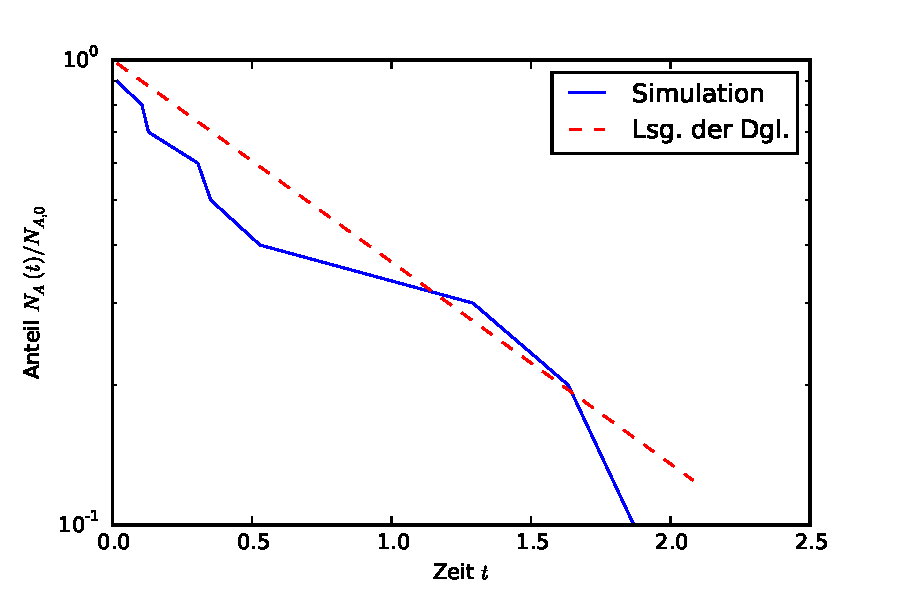
\includegraphics[width=.475\textwidth]{A1n10.pdf}
    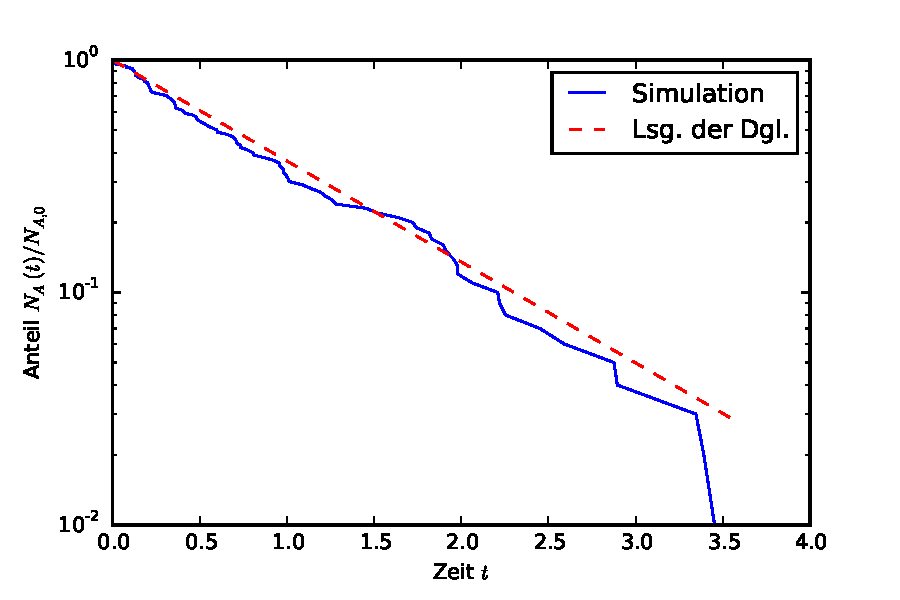
\includegraphics[width=.475\textwidth]{A1n100.pdf}
    \caption{$N_{A, 0} = 10^1$ (links) und $N_{A, 0} = 10^2$ (rechts)}
\end{figure}
\end{minipage}
\begin{minipage}{\textwidth}
\begin{figure}[H]
    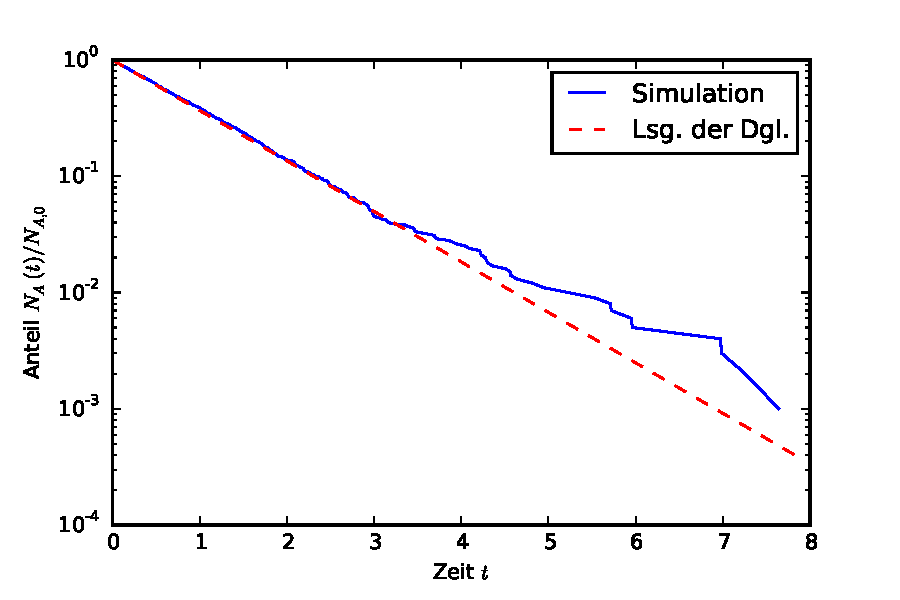
\includegraphics[width=.475\textwidth]{A1n1000.pdf}
    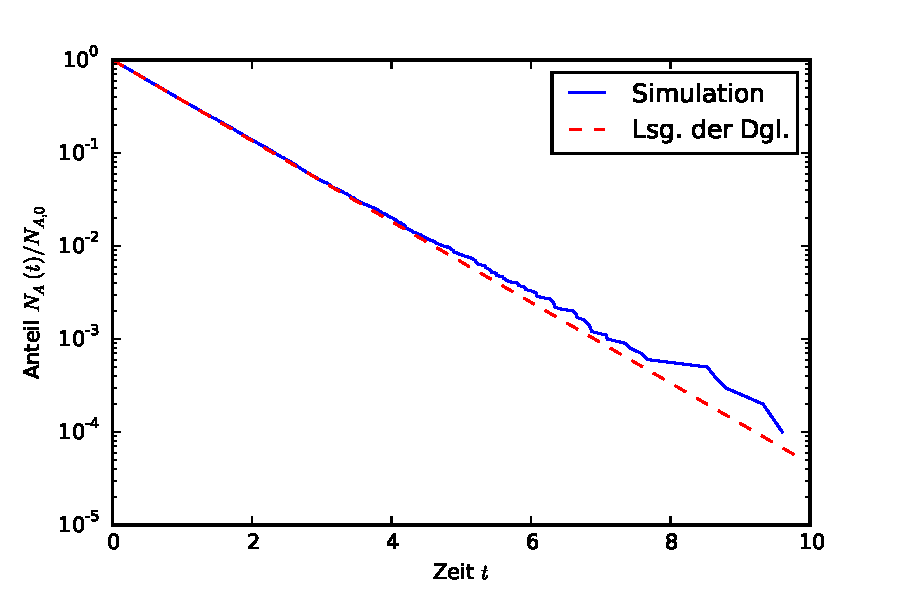
\includegraphics[width=.475\textwidth]{A1n10000.pdf}
    \caption{$N_{A, 0} = 10^3$ (links) und $N_{A, 0} = 10^4$ (rechts)}
\end{figure}
\end{minipage}
\begin{minipage}{\textwidth}
\begin{figure}[H]
    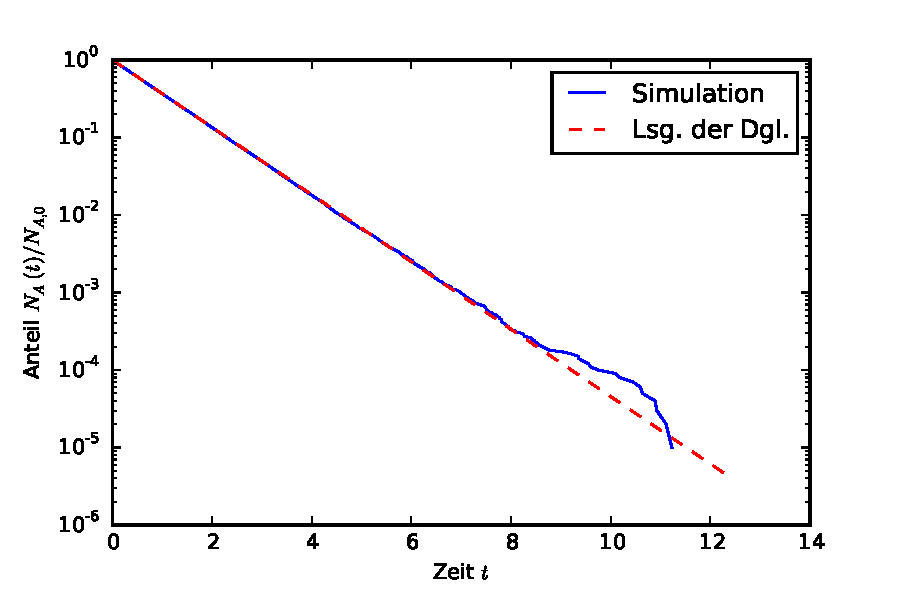
\includegraphics[width=.475\textwidth]{A1n100000.pdf}
    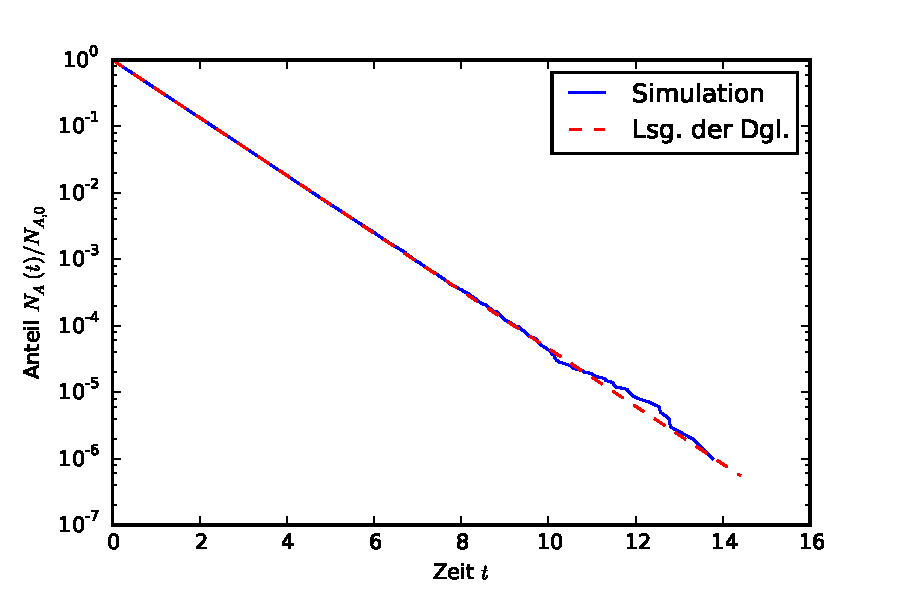
\includegraphics[width=.475\textwidth]{A1n1000000.pdf}
    \caption{$N_{A, 0} = 10^5$ (links) und $N_{A, 0} = 10^6$ (rechts)}
\end{figure}
\end{minipage}

\subsection{*Zusatz: Mittlere Zeit bis zum vollständigen Zerfall}

\newpage

\section{Brusselatormodell}
\subsection{Einleitung}
Das Brusselatormodell ist eine Reaktion mit dynamischer Instabilität und wird durch follgende Reaktion beschrieben: 
\begin{align*}
    &~ R_0: X_0 \rightarrow X_0 + Y_0\\
    &~ R_1: X_1 \rightarrow X_1 + Y_1 + Z_0\\
    &~ R_2: 2Y_0 + Y_1 \rightarrow 3Y_0\\
    &~ R_3: Y_0 \rightarrow Z_1
\end{align*}
Die Teilchen der Sorte $X_i$ sind die Resource der Reaktion. Die Anzahl der Edukte $X_i$ wird konstant gehalten, indem immer, wenn z.B. $X_0$ in $Y_0$ umgewandelt wird, wieder ein $x_0$ Teilchen hinzugefügt wird ($R_0$). Es handelt sich beim Brusselator um ein einfaches Modell chemischer Oszillatoren.

\subsection{Differentialgleichung}

\begin{align*}
    &~ R_0: \frac{dy_0}{dt} = k_0 \cdot x_0 \\
    &~ R_1: \frac{dy_1}{dt} = k_1 \cdot x_1 \\
    &~ R_2: \frac{dy_0}{dt} = k_2 \cdot y_0^2 \cdot y_1;  \frac{dy_1}{dt} = -k_2 \dot y_0^2 \cdot y_1 \\
    &~ R_3: \frac{dy_0}{dt} = -k_3 \cdot y_0\\
    \Rightarrow &~ \frac{dy_0}{dt} = k_0 \cdot x_0 + k_2 \cdot y_0^2\cdot y_1 - k_3 \cdot y_0 \\
    &~ \frac{dy_1}{dt} = k_1 \cdot x_1 - k_2 \cdot y_0^2 \cdot y_1
\end{align*}
Dabei sind $k_0$, $k_1$, $k_2$ und $k_3$ die jeweiligen Reaktionsraten der Reaktionen $R_0, R_1, R_2 und R_3$.









\subsection{Übergangsraten}
\subsection{Simulation}
\dots 
\section{Simulation von Ratenübergängen}
\section{Von Reaktionsraten und Übergangsraten}
\newpage
\section{Wichtige Befehle in Python}
\begin{enumerate}
\item \lstinline[]{np.random.exponential(scale=1.0, size=None)} \\
Draw samples from an exponential distribution. 
\item \lstinline[]{np.random.rand(d0, d1, ..., dn)} \\
Erzeugt gleichverteilte Zufallszahlen im Intervall [0, 1]. Optional können die Dimensionen eines Arrays übergeben werden, so dass eine Matrix mit Zufallszahlen zwischen 0 und 1 zurück gegeben wird. 
\item \lstinline[]{np.argmax(a, axis=None, out=None)[source]} \\
Gibt den Index des Maximums auf einer gegebenen Achse zurück.
\end{enumerate}

\newpage
\section{Quellenverzeichnis}
[1] http://www.uni-magdeburg.de/exph/mathe\_gl/dgl-phys1.pdf

\end{document}
